\part{Implementierungsdetails}
Der Student hatte die Aufgabe im Rahmen seines Praktikums einen
``Gehaltsbenchmark für Mitteldeutschland`` im Bereich  Softwareentwicklung zu
konzeptionieren und umzusetzen. Ziel des Praktikums war der praktische Einatz
der neuen Software für das Unternehmen um dessen Produktpalette zu erweitern.
\section{statistische Berechnungen}
Um die erhaltenen Daten korrekt zu verarbeiten und zu berechnen wurden Formeln
aus der Statistik herangezogen. Folgende Berechnungen wurden für die Auswertung
der Daten getätigt:
\begin{itemize}
  \item Median 
  \item Maximum
  \item Minimum
  \item Mittelwert
  \item oberes Quartil
  \item unteres Quartil
  \item Interquartilsabstand
  \item Ausreißerverdächtige Werte
\end{itemize}
\section{Phasen der Implementierung}
Die Arbeit wurde in drei Phasen gegliedert. 
\begin{enumerate}
  \item Erweiterung des Webservices www.kanaleo.de um das Drupalmodul "Webform"
  \item Verarbeitung und Bereitstellung der Daten mittels Ruby on Rails für die
Javascriptbibliothek Flotr2 
  \item Erstellung der Auswertung in Form eines PDFs, welches an den Kunden
ausgeliefert werden konnte
\end{enumerate}
\subsection{Erwiterung des Webservices www.kanaleo.de}
Zu Beginn der Arbeit wurde vom Autor in zusammenarbeit mit dem Verantwortlichen
Herrn Dr. Jörg Klukas die Erweiterung des Webservices kanaleo.de
vereinbart. Dazu wurde nach einer gründlichen Recherche das Drupalmodul
"Webform" für die Umsetzung des Projektes verwendet. Dieses Modul bot eine
schnelle Entwicklung des Fragebogens. Mittels eines vom Modul bereitgestellten
Baukastens konnten via Drag and Drop alle Elemente der Umfrage Platziert
werden. Nachfolgend sehen Sie einen Auszug der Entwicklung des
Fragebogens.\begin{figure}
 \centering
 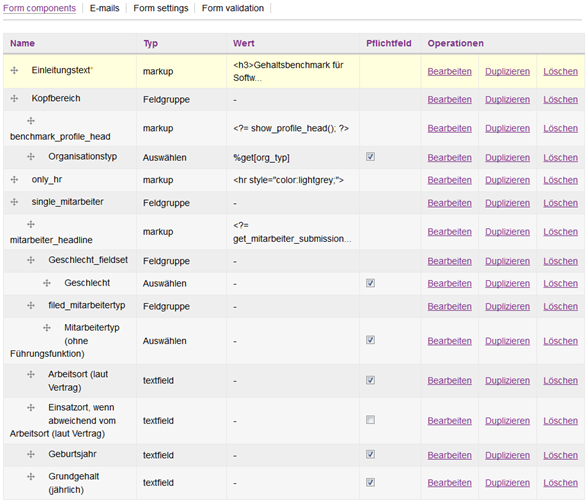
\includegraphics{material/fragebogen.png}
 % fragebogen.png: 588x501 pixel, 96dpi, 15.56x13.26 cm, bb=0 0 441 376
 \caption{Auszug der Entwicklung des Fragebogens mittel des Moduls Webform}
\end{figure}
\newpage 
\subsection{Verarbeitung und Bereitstellung der Daten}
Die Wahl des Studenten fiel bei der Verarbeitung und Bereitstellung der Daten
auf das Framework Ruby on Rails. Der Grund hierfür war, dass das Praktikum
Möglichkeiten zum erlernen neuer Techniken einräumen sollte. Ruby, als Basis
des Frameworks, ist eine interessante Sprache, die dem Autor viel Raum zur
Umsetzung des Projektes gab. Anhand der nachfolgenden Auszüge des Programmcodes
wird der Student erläutern welche Berechnungen angestellt wurden und in welchem
Format die Daten an die Javascriptbibliothek übergeben werden mussten um
korrekte Diagramme und Grafiken zu erhalten. 
\lstset{language=ruby}
\begin{lstlisting}
def median
    case self.size % 2
    when 0 then self.sort[self.size/2-1,2].mean
    when 1 then self.sort[self.size/2].to_f
    end if self.size > 0            
  end
\end{lstlisting}

\subsection{Erstellung der Auswertung in Form eines PDFs}
Die Auswertung wurde in zwei Teile gegliedert. Der erste Teil ist der 
allgemeine Teil, in dem alle abgegebenen Daten ausgewertet und grafisch
dargestellt werden. Im zweiten Teil geht es um den Teilnehmer persönlich. Das
heiß, Die Daten des teilnehmenden Unternehmens werden ausgewertet und mit allen
anderen Werten verglichen. So erhält man eine gute Übersicht über die
Ergebnisse. Die erstellung des PDFs erfolgte mittels
''wkhtmltopdf''\footnote{http://code.google.com/p/wkhtmltopdf/}. Dieses Tool
ist eine simple Shell-Anwendung die es ermöglicht aus einem HTML-Dokument ein
PDF zu generieren. Dabei nutzt das Tool webkit\footnote{http://www.webkit.org/}
und qt\footnote{http://qt.nokia.com/products/}. Das im
\fullref{sec:entwurf} erwähnte Bezahlmodell wird nachfolgend anhand von
Screenshots der Auswertung näher erläutert. 
